\documentclass{beamer}
\usetheme{Boadilla}
\usecolortheme{crane}
%\usefonttheme[stillsansseriflarge, stillsansserifsmall]{serif}
\usefonttheme[stillsansseriflarge, stillsansserifsmall]{structurebold}
\usefonttheme[onlymath]{serif}
\useinnertheme{default}

\usepackage{fontspec}
%\usepackage{kpfonts}
%\setmainfont[Numbers=OldStyle]{Tex Gyre Pagella}
\setsansfont[BoldFont=tintin.ttf]{tintin_talking.ttf}

\usepackage[frenchb]{babel}


%proper math and math symbols
%\usepackage{amsmath}
\usepackage{amssymb}

\usepackage{siunitx}
\usepackage{booktabs}
\usepackage{multirow}

% Allow the usage of graphics (.jpg, .png, etc.) in the document
\usepackage{graphicx}
\usepackage{tikz}
\usetikzlibrary{arrows,shapes,backgrounds, positioning, intersections, decorations.markings, mindmap, shapes.geometric, matrix, shapes.callouts}

\usepackage{pgfplots}
%\usepgfplotslibrary{units}
\usepgfplotslibrary{groupplots}
\usepgfplotslibrary{external}
\tikzset{external/system call={lualatex \tikzexternalcheckshellescape -halt-on-error -interaction=batchmode -jobname "\image" "\texsource"}}

\tikzexternalize

%bibliography
\usepackage{natbib}
%\usepackage{bibentry}
\def\newblock{\hskip .11em plus .33em minus .07em}

\institute{ENS Lyon}
\title{Réunion hebdomadaire}
%\subtitle{Rhéologue de Yaourtière !}
\titlegraphic{\begin{tikzpicture}%
\node[inner sep=0] (haddock) {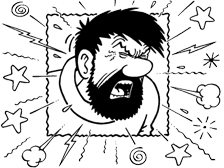
\includegraphics[width=2cm]{haddock}};
\node[rectangle callout, draw, callout relative pointer={(-1,-1)}, 
above right=1 and -1 of haddock] {Rhéologue de Yaourtière !};
\end{tikzpicture}}

\author[M. Leocmach]{Mathieu Leocmach}
\date{5 Dec 2012}

\begin{document}
\tikzset{every mark/.append style={scale=0.8}}
\pgfplotsset{every axis/.append style={small}}
\tikzset{external/force remake=false}

\AtBeginSection[]{
	\addtocounter{framenumber}{-1}
	\begin{frame}[plain]
		\tableofcontents[currentsection, hideothersubsections]
	\end{frame}
}

\begin{frame}[plain]
	\titlepage
\end{frame}

\begin{frame}<1>[label=orga]{Organisation}
\begin{center}
\begin{tikzpicture}
	\node (pic) {%
		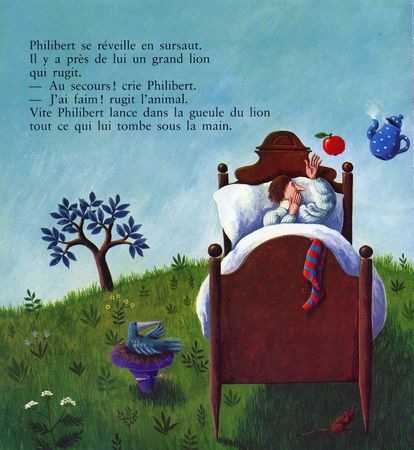
\includegraphics[height=0.7\textheight]{philibert_0}%
		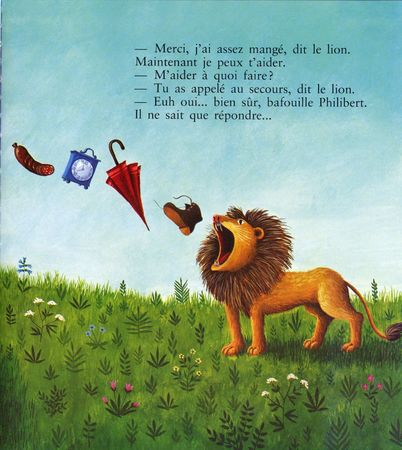
\includegraphics[height=0.7\textheight]{philibert_1}%
	};
	\node at (-1.5,2){Thibaut};
	\node at (3.5,1){\alt<1>{Rhéomètre}{Moi}};
	\node at (-3.5,0.5){\alt<1>{Moi}{Vous}};
\end{tikzpicture}
\end{center}
\end{frame}

\begin{frame}{Gel de Caséine : \og Yaourt \fg{}}
\begin{columns}
\column{0.5\textwidth}
\begin{tabular}{@{}ll@{}}\toprule
Eau &  \\ 
Caseinate de sodium & 4\% \\ 
$\delta$-gluconolactone (GDL) & 1\% \\ 
Billes de polyamides & 3\% \\ 
\bottomrule
\end{tabular}

\bigskip

Pas de gras, pas de ``vrai lait''.
\column{0.5\textwidth}
\begin{itemize}
\item La GDL s'ouvre et acidifie progressivement le milieu.
\item Sous pH=5.5 gélification de la caséine.
\item Les billes sont là comme agent de contraste pour les ultrasons.
\end{itemize}
\end{columns}
\end{frame}
\tikzset{external/force remake=true}
\begin{frame}{Prise et cassure}
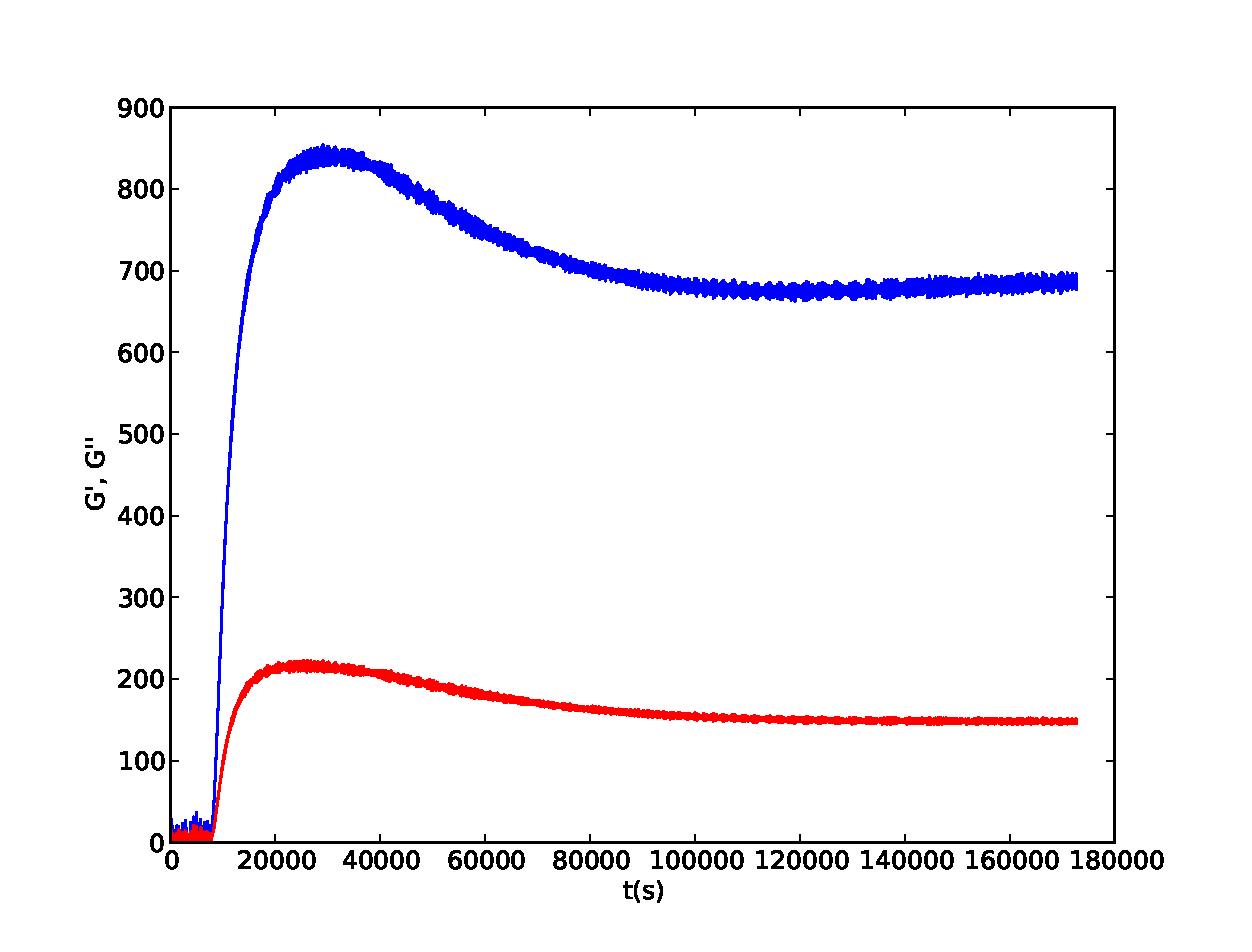
\includegraphics[width=0.5\textwidth]{Y22_prise.eps}%
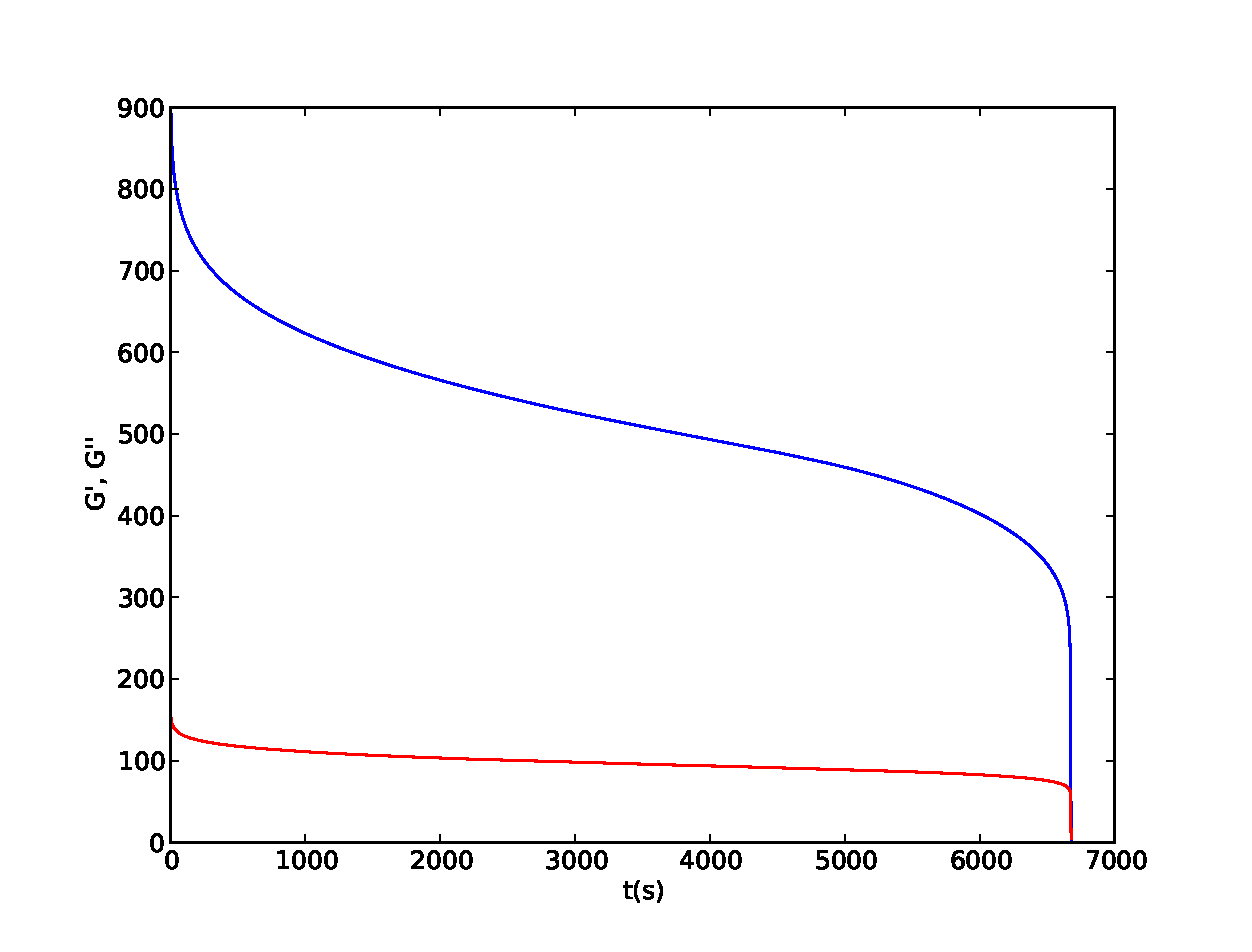
\includegraphics[width=0.5\textwidth]{Y22_rupture.eps}

\begin{itemize}
	\item Prise en \SI{20000}{\second}
	\item Casse en oscillation
	\item Stress imposé (ici \SI{250}{\pascal})
\end{itemize}
\end{frame}
\tikzset{external/force remake=false}
\againframe<2>{orga}

\begin{frame}{Que tirer (de nouveau) des ultrasons ?}
Mesure locale de la déformation du système.
\begin{itemize}
\item Au sein d'une période
\begin{itemize}
	\item Non linéarité ? (LAOS)
	\item Rhéo-épaississant / fluidifiant
	\item Instant de la cassure
\end{itemize}
\item Entre les périodes
\begin{itemize}
	\item Synchronisation rhéomètre-ultrasons
	\item Mesure des déformations irréversibles
	\item Événements plastiques
	\item Comment se prépare la cassure ?
\end{itemize}
\end{itemize}
\end{frame}



\begin{frame}{Vélocimétrie du chatoiement ultrasonore}
(Ultrasonic Speckle Velocimetry)

\begin{tikzpicture}
\pgfplotsset{every axis/.append style={
	height=0.4\textheight,
	xlabel={Temps de retour (\si{\micro\second})},
	ylabel={Intensité}, ymin=-100, ymax=100,
	no marks,
	}}
\pgfplotstableread{speckles.data}\speckles
\begin{axis}[
	name=all,
	anchor=below south west,
	width=\textwidth,
	xmin=13.9,xmax=16.1,
	]
	\fill[gray!10] (axis cs:14.156,-100) rectangle (axis cs:14.284,100)
	(axis cs:15.82,-100) rectangle (axis cs:15.948,100);
	\addplot table[x index=0, y index=1]{\speckles};
	\addplot table[x index=0, y index=2]{\speckles};
	\begin{scope}[inner sep=0]
		\node at (axis cs:14.156,-100) (a){};
		\node at (axis cs:14.284,-100) (b){};
		\node at (axis cs:15.82,-100) (c){};
		\node at (axis cs:15.948,-100) (d){};
	\end{scope}
\end{axis}
\pgfplotsset{every axis/.append style={
	width=0.48\textwidth,
	}}
\begin{axis}[%
	xmin=14.156,xmax=14.284,
	xtick={14.15,14.20,...,14.40},
	anchor=above north west,
	at={(0,-1)},
	name=A,
	]
	\addplot table[x index=0, y index=1]{\speckles};
	\addplot table[x index=0, y index=2]{\speckles};
	\draw[->] (axis cs:14.2,50) -- (axis cs:14.205,50);
\end{axis}
\begin{axis}[%
	xmin=15.82,xmax=15.948,
	xtick={15.8,15.85,...,16},
	anchor=above north east,
	at={($(all.below south east)+(0,-1)$)},
	name=B,
	]
	\addplot table[x index=0, y index=1]{\speckles};
	\addplot table[x index=0, y index=2]{\speckles};
	\draw[->] (axis cs:15.895,50) -- (axis cs:15.91,50);
\end{axis}
\draw[dotted] (a)--(A.north west) (A.north east)--(b)
	(c)--(B.north west) (B.north east)--(d);
\end{tikzpicture}
\end{frame}

\begin{frame}{Sur une période}
\begin{columns}
\column{0.5\textwidth}
\begin{tikzpicture}
\begin{axis}[%
	width=\columnwidth,
	xmin=13.9,xmax=16.098,
	ymin=0,ymax=5000,
	y dir=reverse, ylabel={\#tir},
	xlabel={Temps de retour (\si{\micro\second})}
	]
	\addplot graphics[
		xmin=13.9,xmax=16.098,
		ymin=0,ymax=5000,
		]{speckles_1oscil};
\end{axis}
\end{tikzpicture}
\column{0.5\textwidth}
\begin{itemize}
\item Déplacement entre deux tirs successifs
\begin{itemize}
\item à tout instant
\item en tout endroit du gap
\end{itemize}
\item LAOS local
\begin{itemize}
\item Transformée de Fourier
\item Amplitude et phase des premières harmoniques
\end{itemize}
\end{itemize}
\end{columns}
\end{frame}

\begin{frame}{Amplitude des oscillations lors de la rupture}
\tikzset{external/force remake=false}%
\begin{columns}
\column{0.5\textwidth}
\begin{tikzpicture}
\begin{axis}[%
	width=\columnwidth,
	height=\columnwidth,
	xmin=14.4,xmax=16.4,
	ymin=0,ymax=414,
	y dir=reverse, ylabel={\#tir},
	xlabel={Temps de retour (\si{\micro\second})}
	]
	\addplot graphics[
		xmin=14.4,xmax=16.4,
		ymin=0,ymax=414,
		]{Y22_I1.png};
\end{axis}
\end{tikzpicture}
\column{0.5\textwidth}
Mais
\begin{itemize}
\item Linéaire après la rupture
\item Beaucoup de bruit avant la rupture
\end{itemize}
$\Rightarrow$ pas possible de faire du LAOS
\begin{tikzpicture}
\begin{axis}[%
	width=\columnwidth,
	height=0.5\columnwidth,
	xmin=14.4,xmax=16.4,
	ymin=0,ymax=68,
	y dir=reverse, ylabel={\#tir},
	xlabel={Temps de retour (\si{\micro\second})}
	]
	\addplot graphics[
		xmin=14.4,xmax=16.4,
		ymin=0,ymax=68,
		]{Y22_I1_avantrupture.png};
\end{axis}
\end{tikzpicture}
\end{columns}
\end{frame}

\begin{frame}{Entre deux oscillations}
\begin{columns}
\column{0.5\textwidth}
\includegraphics[width=\columnwidth]{av_irr_tir0-16.eps}
\column{0.5\textwidth}
Conceptuellement la même chose qu'au cours d'un cycle, mais on regarde l'irréversibilité.
\begin{itemize}
\item Beaucoup de bruit, sauf à la rupture
\item Nécessaire de moyenner sur 5 tirs avant corrélation
\end{itemize}
\end{columns}

%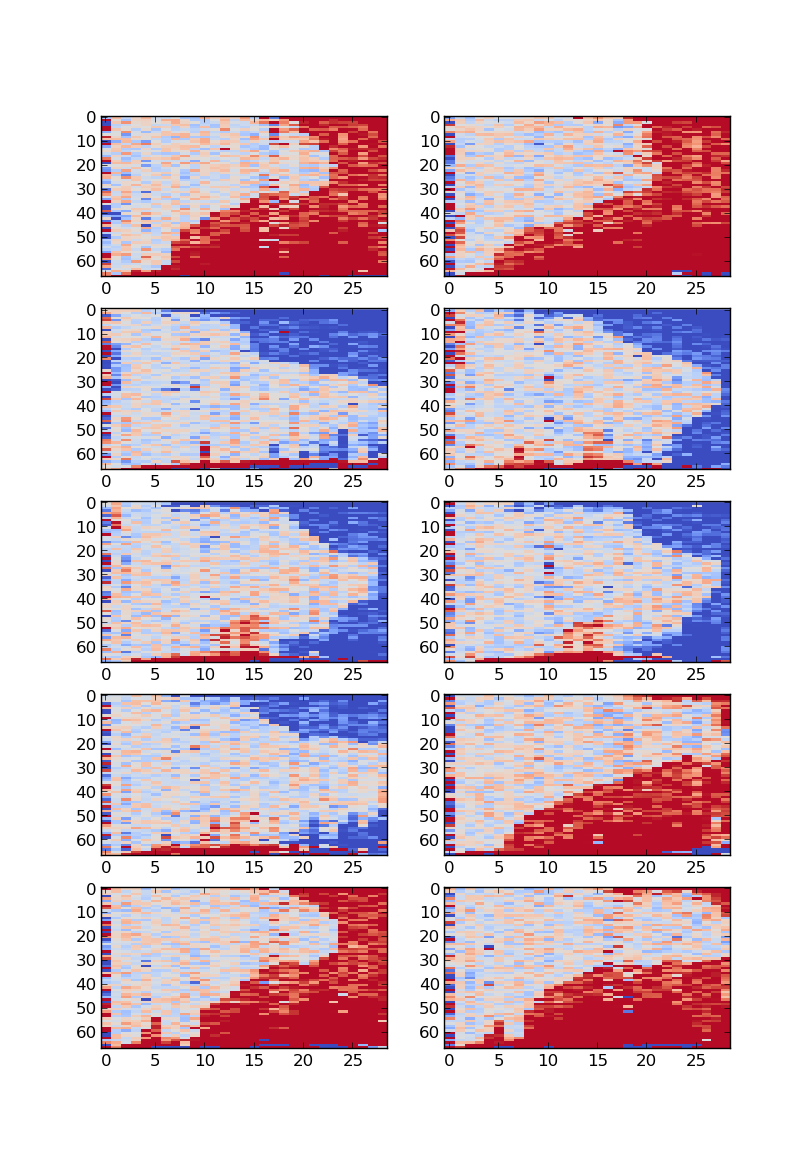
\includegraphics[width=\columnwidth]{irr_av5.png}

\end{frame}

\begin{frame}{Ca fait mal aux yeux, hein ?}
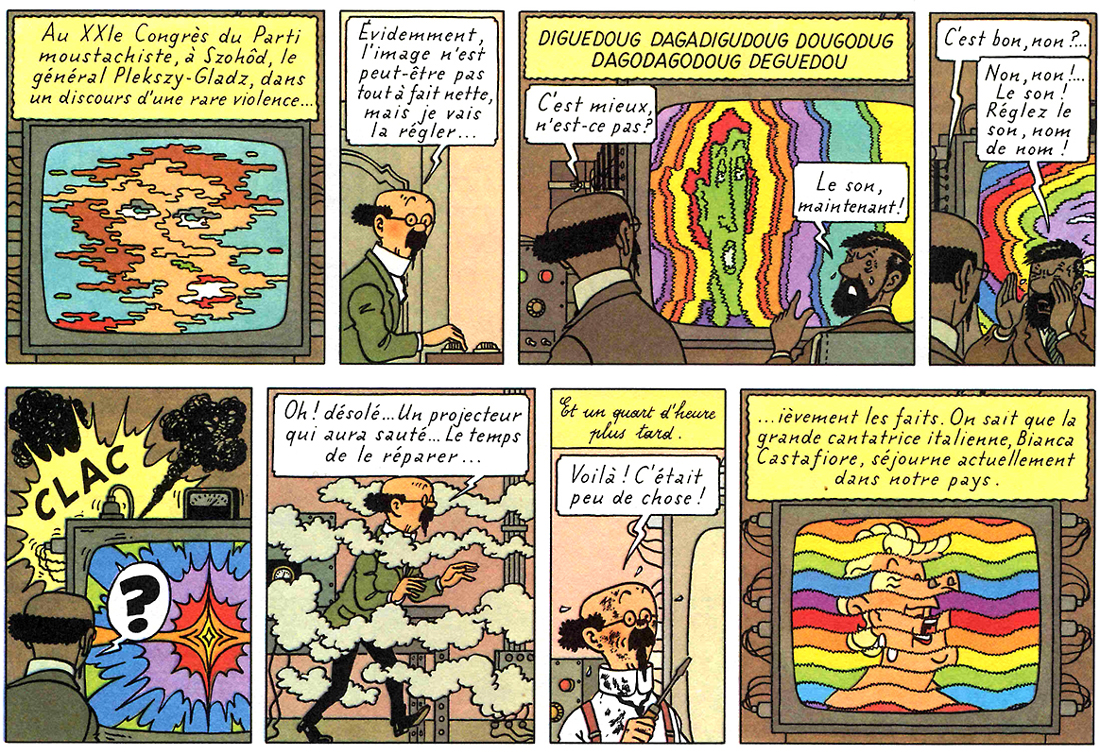
\includegraphics[width=\columnwidth]{TV_tournesol.jpg}
\end{frame}

\begin{frame}{Au cours du cycle}
\begin{columns}
\column{0.5\textwidth}
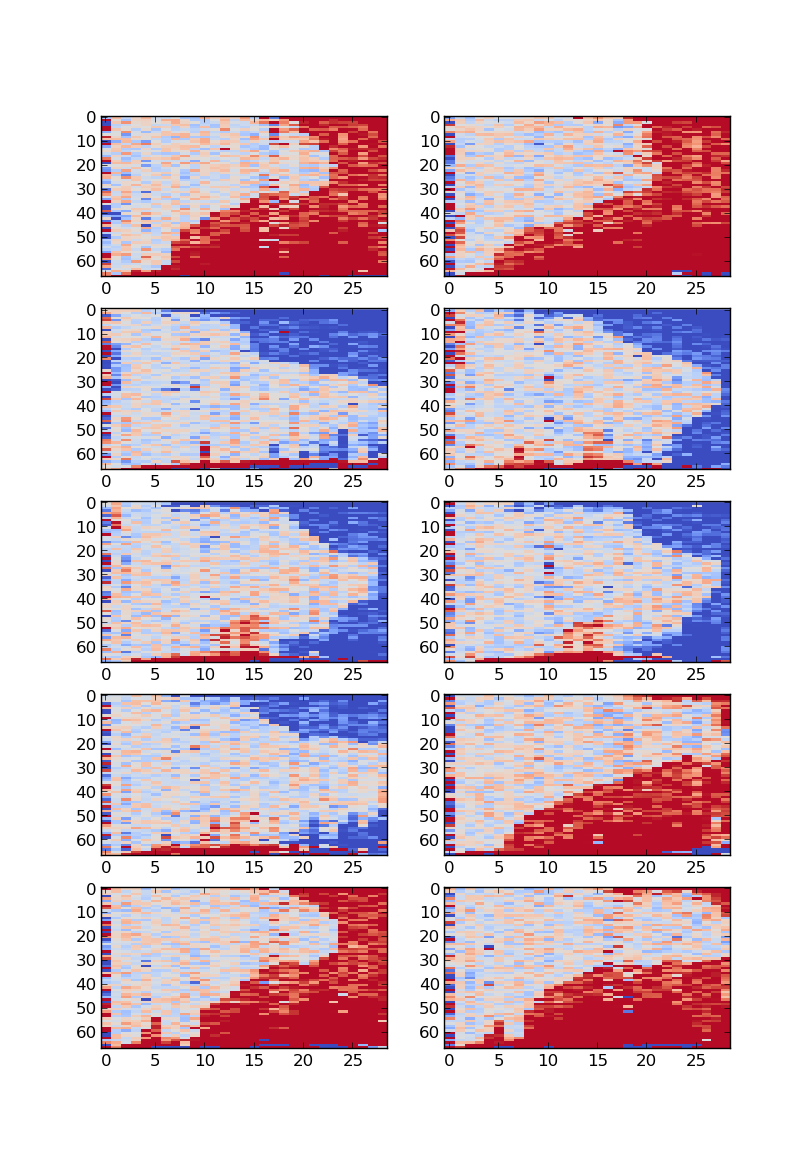
\includegraphics[width=\columnwidth]{irr_av5.png}
\column{0.5\textwidth}
\begin{itemize}
\item On voit bien le changement de sens de l'oscillation
\item Certains endroits du gap se déplacent à contre-sens
\item 3D !
\end{itemize}
\end{columns}
\end{frame}

\begin{frame}
\begin{itemize}
\item Très difficile d'obtenir quoi que ce soit sur une manip plus longue
\item Trop de bruit
\item C'est le même problème que les déplacements au cours d'un seul cycle
\item Si on compare deux speckles ``trop proches'' on ne trouvera que du bruit
\item Ce bruit s'intègre en bruit et pas en signal
\item Pas possible de corréler puis flouter
\end{itemize}
$\Rightarrow$ Chercher un moyen de ne comparer que des speckles ``assez éloignés'' pour ne pas avoir de bruit.
\end{frame}

\end{document}